\subsection{Overview}
The TrackMe services are built on a client-server structure, this way the system is organized through abstraction levels.
We chose to adopt a 3-tier architecture:
\begin{itemize}
	\item \textbf{Presentation Tier} \\This layer makes the interaction possible between the user and the system. Here the user sees all the information provided by the system in a easily way to understand them.
	\item \textbf{Application Tier} \\This layer is managed almost totally by Data4Help service that is in charge of:
	\begin{itemize}
		\item store data incoming from the external;
		\item collect data information from database in order to execute Third parties’ requests;
		\item also generates data statistics on data collected;
		\item send to third parties requested data.
	\end{itemize}
	Moreover even AutomatedSOS has logic application in order to continuously monitor users’ health status.
	\item \textbf{Data Tier} \\In this layer all the sensible users’ data (location, health status) are stored into Databases and are retrieved by the application tier in order to do statistics and answer third parties’ requests.
\end{itemize}

More specifically Data4Help manage the data and core logic sections while AutomatedSOS and Track4Run manage the presentation section. Actually, a small part of application tier is also present in AutomatedSOS, this is due to the fact that the Health Monitoring process requires to be executed as fast as possible.

\subsection{Component View}
\subsection{Deployment View}
The following Deployment Diagram captures the topology of the system's hardware.
The SmartphoneApp and SmartWatchApp (Presentation Tier) communicate to the Application Server through RMI, while the WebBrowser communicates to the WebServer through HTTP protocol. The Application Server (Application Tier) communicates to the Database Server (Data Tier) through JDBC.

\begin{figure}[H]
\centering
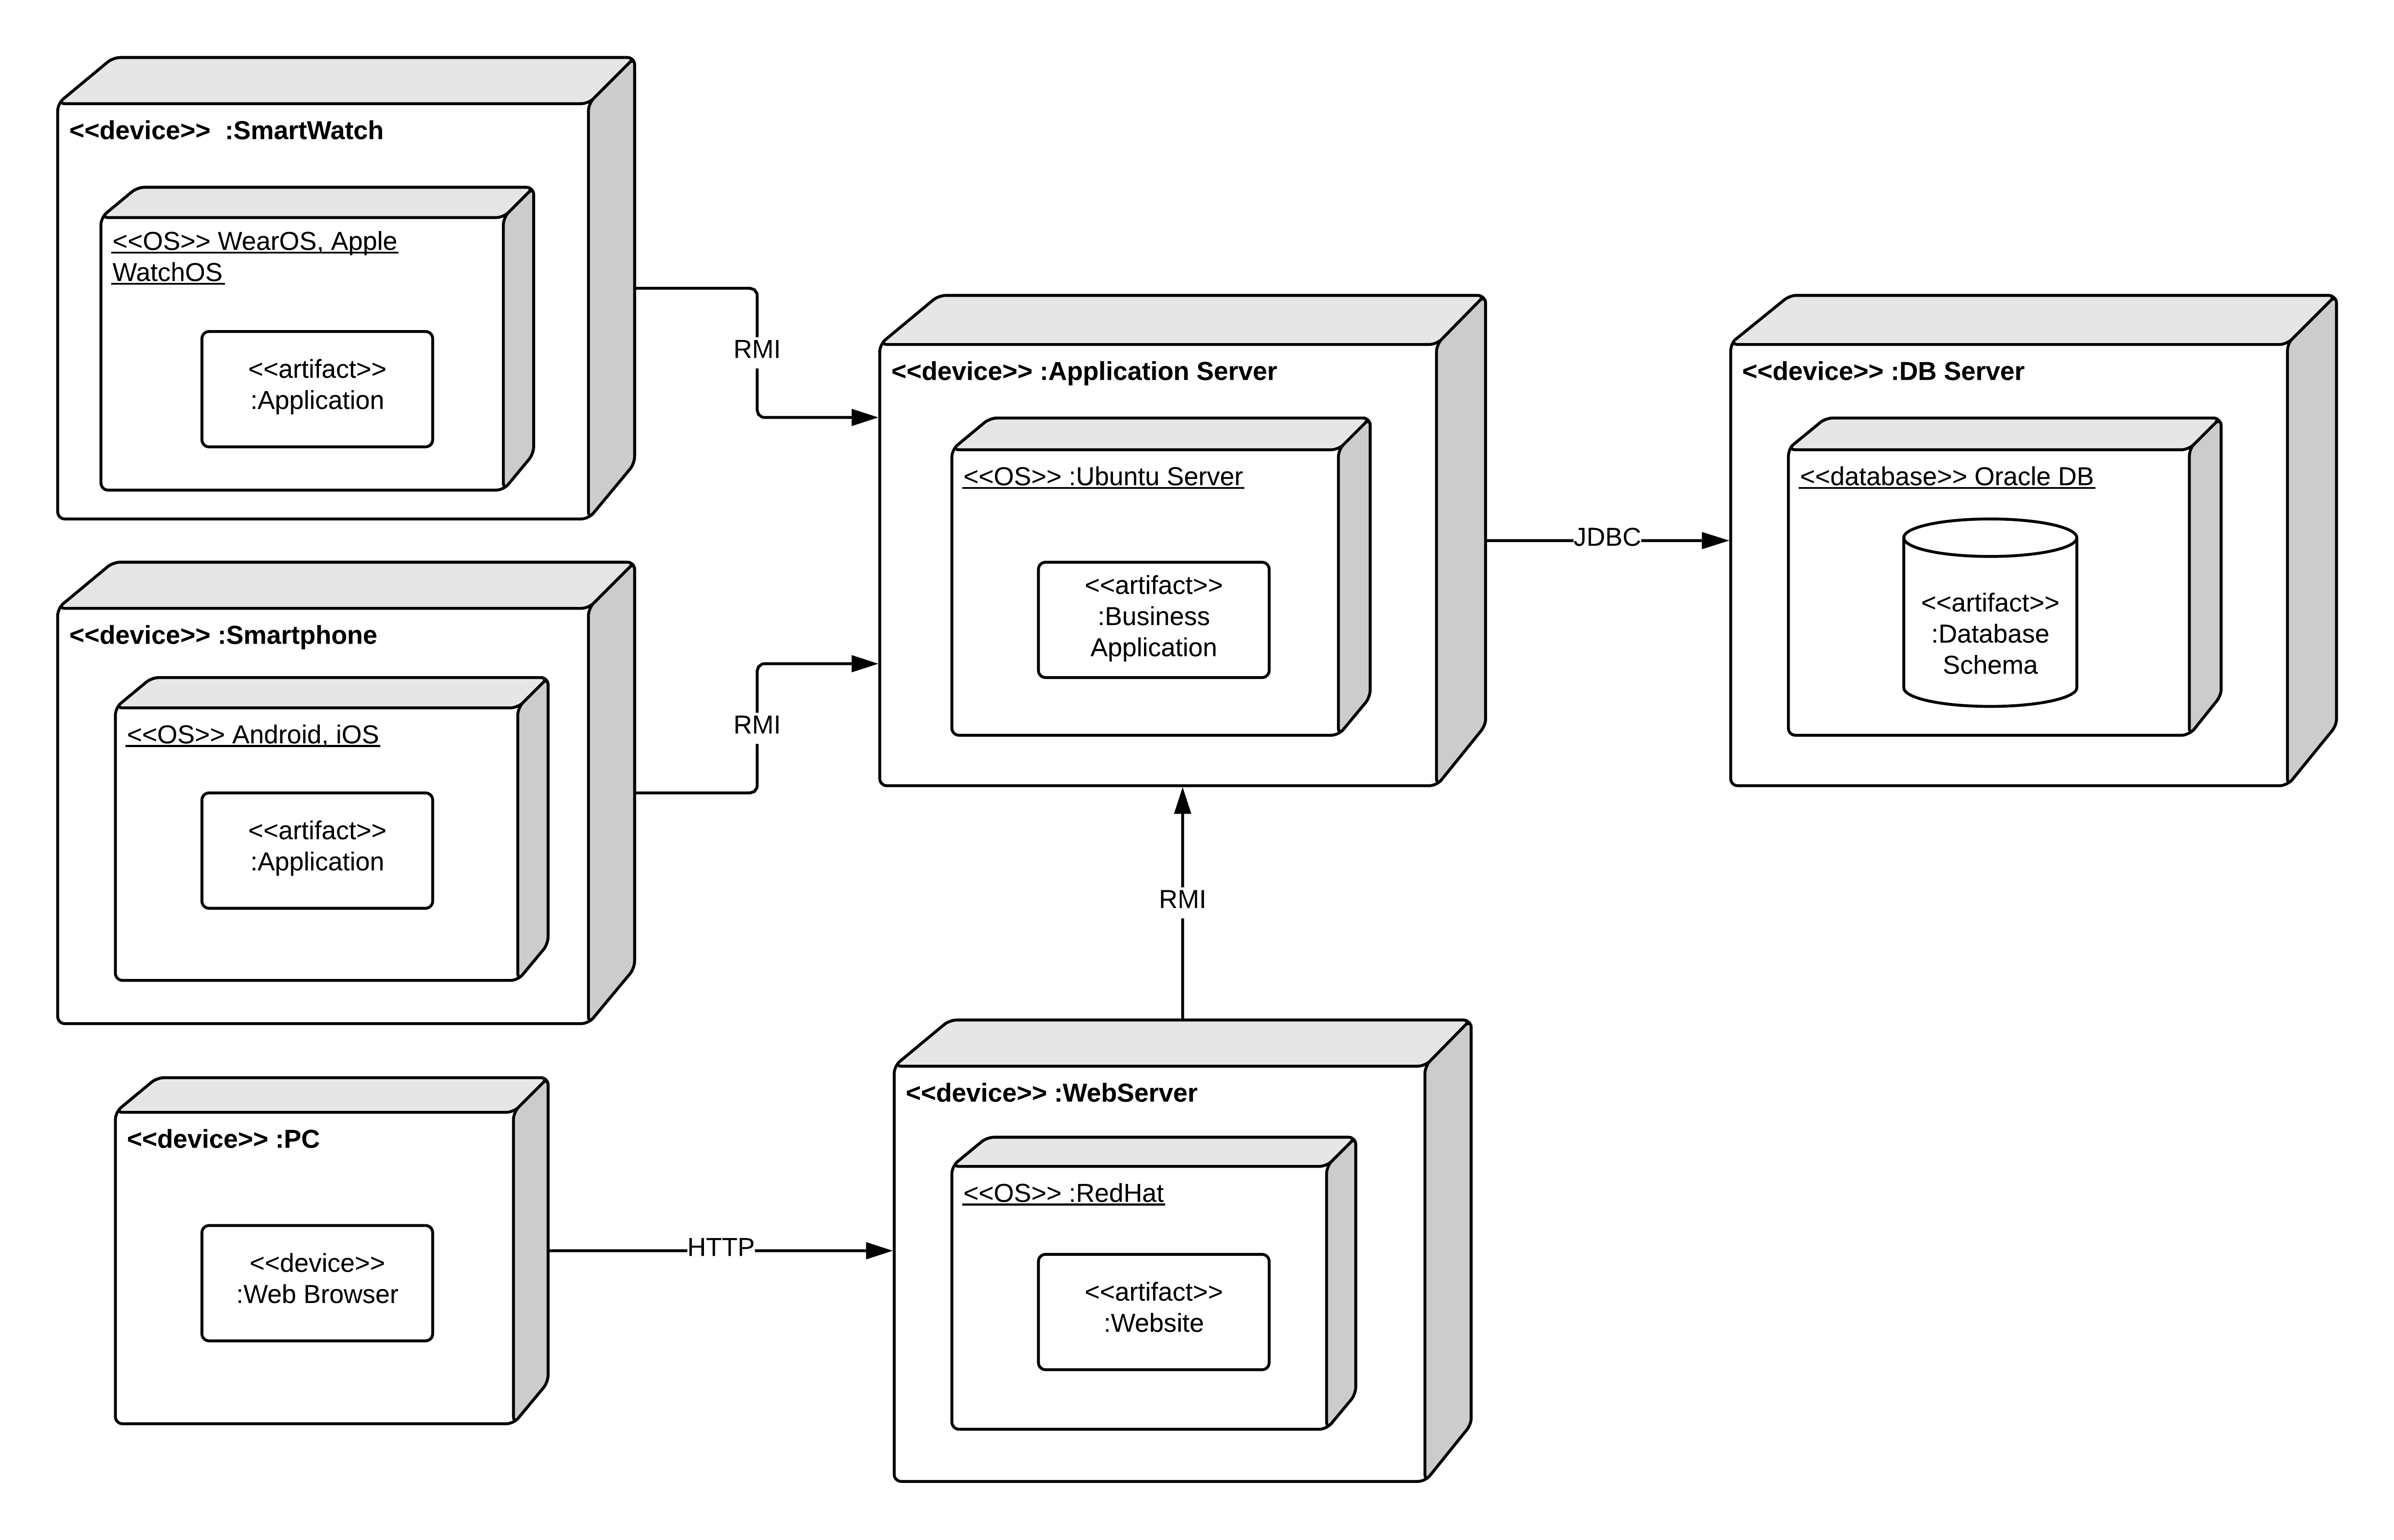
\includegraphics[scale=0.35]{Images/DeploymentDiagram.png}
\caption{Deployment Diagram.}
\end{figure}

\subsection{Runtime View}
\subsection{Component Interfaces}
\subsection{Selected Architectural Styles and Patterns}
\subsection{Other Design Decisions}